U.S. Department of Homeland Security\\
Citizenship and Immigration Services\\
\strut \\
RE: EB-2 Petition for Permanent Residency with request for a National Interest Waiver

\begin{center}
Petitioner/Beneficiary: \quad Mr. \myname \\
Type of Petition: \quad Form I-140\\
Classification Sought: \quad INA §203(b)(2)(B)\\
\strut \\
National Interest Waiver Petition Letter
\end{center}

Dear Immigration Officer:\\
\strut \\
This petition is respectfully submitted in support of Mr. \myname's application for classification as a qualified immigrant under the preference of advanced degree professional/alien of exceptional ability. The evidence submitted herewith will specifically demonstrate that Mr. \myname qualifies for a National Interest Waiver under the standards set by Matter of Dhanasar, 26 I\&N Dec. 884 (AAO 2016).\\
\strut \\
Specifically, the evidence submitted will prove that:\\
1. Mr. \myname is a member of the professions holding an advanced degree;\\
2. Mr. \myname's proposed endeavor has both substantial merit and national importance;\\
3. Mr. \myname is well positioned to advance the proposed endeavor; and\\
4. On balance, it would be beneficial to the United States to waive the
requirements.

\emph{Note that the standard of proof for petitions filed for National
Interest Waiver cases is the ``preponderance of the evidence'' standard.
See Matter of Dhanasar, 26 I\&N Dec. 884, 889 (AAO 2016). Thus, if the
petitioner submits relevant, probative, and credible evidence that leads
USCIS to believe that the claim is ``more likely than not'' or
``probably true,'' the petitioner has satisfied the standard of proof.
Matter of E-M-, 20 I\&N Dec. 77, 79-80 (Comm'r 1989); see also U.S. v.
Cardoza-Fonseca, 480 U.S. 421 (1987) (discussing ``more likely than
not'' as a greater than 50\% chance of an occurrence taking place).}

\newpage

\section{\red{Exhibit Commands Usage Examples (Remove This Section in Final Submission)}}

\vspace{5mm}
\textbf{1. Create an exhibit with an index and label}
\begin{verbatim}
\exhibittext{cv}{1}{CV of Mr. XXXX.}
\end{verbatim}
where "cv" is the label, "1" is the index, and "CV of Mr. XXXX." is the text after the index. It'll be like
\exhibittext{cv}{1}{CV of Mr. XXXX.}.

\vspace{5mm}
\textbf{2. Create an exhibit with an index only}
\begin{verbatim}
\exhibittext{cv-without-lalel}{2}{}.
\end{verbatim}
It'll be like \exhibittext{cv-without-lalel}{2}{}.

\vspace{5mm}
\textbf{3. Refer to an existing exhibit Fully}
\begin{verbatim}
\refexhibit{cv}.
\end{verbatim}
It'll be like \refexhibit{cv}. Note that there are no parentheses here.

\vspace{5mm}
\textbf{4. Refer to an existing exhibit's index}
\begin{verbatim}
\refexhibitnum{cv}.
\end{verbatim}
It'll be like \refexhibitnum{cv}.

%%%%%%%%%%%%%%%%%%%%%%%%%%%%%%%%%%%%%%%%%%%%%%%%%%%%%%%%%
\section{\texorpdfstring{1. MR. \myname IS A MEMBER OF THE PROFESSIONS HOLDING AN ADVANCED DEGREE}{1. MR. \myname IS A MEMBER OF THE PROFESSIONS HOLDING AN ADVANCED DEGREE}}\label{mr.-xxx-is-a-member-of-the-professions-holding-an-advanced-degree}


\exhibittext{ms-in-cs}{3-1}{the Master of Science degree in Computer Science of Mr. First Last.} Moreover, Mr. \myname had a good academic outstanding with a high GPA of 4.0 \exhibittext{ms-in-cs-gpa}{3-2}{the Official Transcript of Mr. First Last.}.


\section{\texorpdfstring{2. MR. \myname\textquotesingle S PROPOSED ENDEAVOR}{2. MR. \myname'S PROPOSED ENDEAVOR}}\label{mr.-xxx-proposed-endeavor}

\section{\texorpdfstring{3. SUBSTANTIAL MERIT AND NATIONAL IMPORTANCE}{3. SUBSTANTIAL MERIT AND NATIONAL IMPORTANCE}}\label{substantial-merit-and-national-importance}

\subsection{\texorpdfstring{3.1. Mr. \myname's Proposed Endeavor Has Substantial Merit}{3.1. Mr. \myname's Proposed Endeavor Has Substantial Merit}}\label{mr.-xxx-proposed-endeavor-has-substantial-merit}

On February 12, 2024, the White House Office of Science and Technology Policy (OSTP) released an updated list of critical and emerging technologies that are potentially significant to U.S. national security. \exhibittext{white-house-list}{9}{Critical and Emerging Technologies List 2024 Update.}

\subsection{\texorpdfstring{3.2. Mr. \myname's Proposed Endeavor Has National Importance}{3.2. Mr. \myname's Proposed Endeavor Has National Importance}}\label{mr.-xxx-proposed-endeavor-has-national-importance}

\section{\texorpdfstring{4. MR. \myname IS WELL POSITIONED TO ADVANCE THE PROPOSED ENDEAVOR}{4. MR. \myname IS WELL POSITIONED TO ADVANCE THE PROPOSED ENDEAVOR }}\label{mr.-xxx-is-well-positioned-to-advance-the-proposed-endeavor}

Dhanasar indicates that the second prong of the analysis must consider whether the petitioner is well positioned to advance the proposed endeavor (Dhanasar, at 890). This multifactorial assessment includes an evaluation of the petitioner's education, skills, knowledge, and record of success in related efforts; a model or plan for future activities; any progress made toward achieving the proposed endeavor; and the interest of potential customers, users, investors, or other relevant entities or individuals (Id.). Importantly, Dhanasar points out the inherent difficulty in "forecasting feasibility or future success", even in the presence of a cogent plan and competent execution;
therefore, petitioners are not required to show that their proposed endeavor is more likely than not to succeed (Id.). \exhibittext{Dhanasar}{22}{the Matter of DHANASAR, Petitioner, 26 I\&N Dec. 884 (AAO 2016)}

\subsection{\texorpdfstring{4.1. Education, Skills, and Knowledge}{4.1. Education, Skills, and Knowledge}}\label{education-skills-and-knowledge}

\subsection{\texorpdfstring{4.2. Mr. \myname has been recognized by the academia}{4.2. Mr. \myname has been recognized by the academia}}\label{mr.-xxx-has-been-recognized-by-the-academia}

\subsection{\texorpdfstring{4.3. Record of Success in Related or Similar Efforts and Interest of Potential Customers, Users, Investors, and Other Relevant Individuals}{4.3. Record of Success in Related or Similar Efforts and Interest of Potential Customers, Users, Investors, and Other Relevant Individuals}}\label{record-of-success-in-related-or-similar-efforts-and-interest-of-potential-customers-users-investors-and-other-relevant-individuals}

\subsubsection{\texorpdfstring{4.3.1. Mr. \myname's research has been published in some of the top conferences and journals in the field}{4.3.1. Mr. \myname's research has been published in some of the top conferences and journals in the field }}\label{mr.-xxx-research-has-been-published-in-some-of-the-top-conferences-and-journals-in-the-field}

\subsubsection{\texorpdfstring{4.3.2. Researchers from around the world have applied upon Mr. \myname\textquotesingle{}s research to further their own research }{ 4.3.2. Researchers from around the world have applied upon Mr. \myname's research to further their own research }}\label{researchers-from-around-the-world-have-applied-upon-mr.-xxx-research-to-further-their-own-research}

\begin{figure}
    \centering
    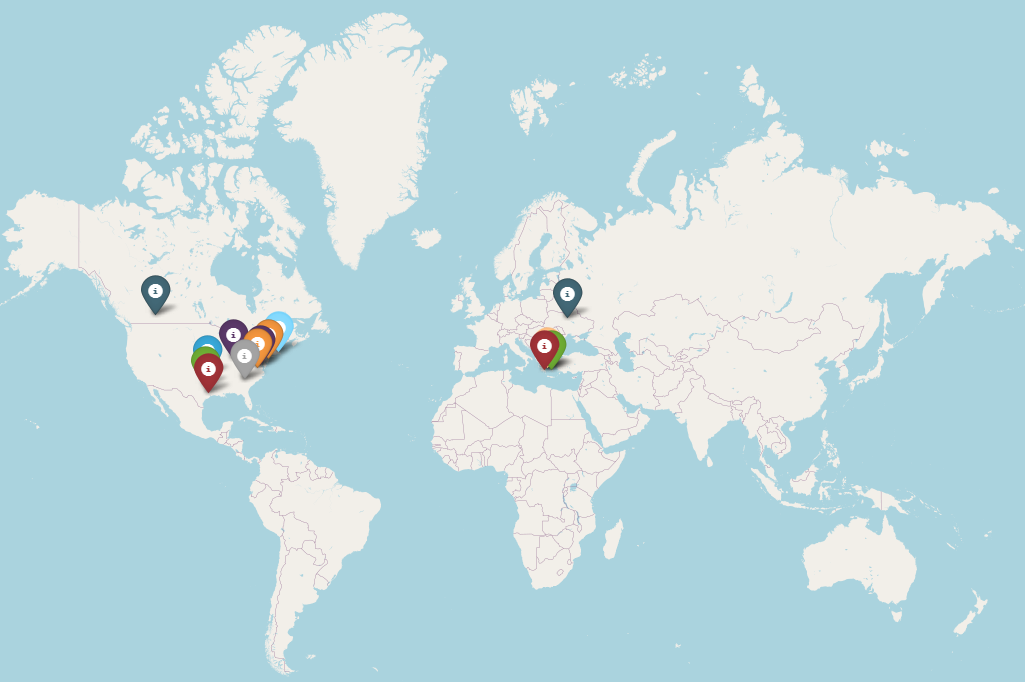
\includegraphics[width=6in,height=3.2in]{map_screenshot.png}
    \caption{The worldwide citation map of Mr. \myname's work.}
    \label{fig:citation_map}
\end{figure}

The citation map can be generated from this Github Repo\footnote{https://github.com/ChenLiu-1996/CitationMap}.

\subsubsection{\texorpdfstring{4.3.3. Mr. \myname served as a reviewer of others\textquotesingle{} research work}{4.3.3. Mr. \myname served as a reviewer of others' research work}}\label{mr.-xxx-served-as-a-reviewer-of-others-research-work}

\subsubsection{\texorpdfstring{4.3.4. Mr. \myname is the awardee of the Fellowships for Graduate Research}{4.3.4. Mr. \myname is the awardee of the Fellowships for Graduate Research}}\label{mr.-xxx-is-the-awardee-of-the-cahmp-summer-fellowships-for-graduate-research}

\subsubsection{\texorpdfstring{4.3.5. Mr. \myname\textquotesingle{}s research is highly novel and influential in the field}{4.3.5. Mr. \myname's is highly novel and influential in the field}}\label{mr.-xxx-research-is-highly-novel-and-influential-in-the-field}

\subsubsection{\texorpdfstring{4.3.6. Mr. \myname\textquotesingle{}s significant original contributions are evident from renowned media}{4.3.6. Mr. \myname's significant original contributions are evident from renowned media}}\label{mr.-xxx-significant-original-contributions-are-evident-from-renowed-media}

\subsubsection{\texorpdfstring{4.3.7. Mr. \myname continuously contributes to U.S. National Science Foundation (NSF) projects}{4.3.7. Mr. \myname continuously contributes to U.S. National Science Foundation (NSF) projects}}\label{mr.-xxx-continuously-contributes-to-us-national-science-foundation-projects}


\subsubsection{\texorpdfstring{4.3.8. Mr. \myname's research and innovations are extensively adopted by users, researchers, and companies}{4.3.8. Mr. \myname's research and innovations are extensively adopted by users, researchers, and companies}}\label{mr.-xxx-research-and-innovations-are-extensively-adopted-by-users-researchers-and-companies}

\subsubsection{\texorpdfstring{4.3.9. Progress toward achieving the proposed endeavor}{4.3.9. Progress toward achieving the proposed endeavor}}\label{progress-toward-achieving-the-proposed-endeavor}

\subsubsection{\texorpdfstring{4.3.10. Plan for future activity in the field}{4.3.10. Plan for future activity in the field}}\label{plan-for-future-activity-in-the-field}

\section{\texorpdfstring{5. ON BALANCE, IT WOULD BE BENEFICIAL TO THE UNITED STATES TO WAIVE THE REQUIREMENTS}{5. ON BALANCE, IT WOULD BE BENEFICIAL TO THE UNITED STATES TO WAIVE THE REQUIREMENTS}}\label{on-balance-it-would-be-beneficial-to-the-united-states-to-waive-the-requirements}

\subsection{\texorpdfstring{5.1. The Significant Benefit of Waiving the Labor Certification Requirement}{5.1. The Significant Benefit of Waiving the Labor Certification Requirement}}


\subsection{\texorpdfstring{5.2. National Interest and Public Benefit}{5.2. National Interest and Public Benefit}}

\subsection{\texorpdfstring{5.3. Economic Impact and Industry Growth}{5.3. Economic Impact and Industry Growth}}

\subsection{\texorpdfstring{5.4. Expertise Beyond Ordinary Training and Value Over Local Workforce}{5.4. Expertise Beyond Ordinary Training and Value Over Local Workforce}}
% ### **Expertise Beyond Ordinary Training and Value Over Local Workforce**


\subsection{\texorpdfstring{5.5. Transdisciplinary Contributions Beyond a Single Employer}{5.5. Transdisciplinary Contributions Beyond a Single Employer}}


\subsection{\texorpdfstring{5.6. Non-Competition with Local Workforce}{5.6. Non-Competition with Local Workforce}}

\subsection{\texorpdfstring{5.7. Reasonability of Waiving PERM and Self-Petition}{5.7. Reasonability of Waiving PERM and Self-Petition}}

\subsection{\texorpdfstring{5.8. Timely Contribution to Emerging Technologies}{5.8. Timely Contribution to Emerging Technologies}}

\subsection{\texorpdfstring{5.9. Unique Expertise and Critical Need}{5.9. Unique Expertise and Critical Need}}

Considering the above factors and the evidence presented therein, Mr.\myname satisfies this prong.

\section{\texorpdfstring{6. CONCLUSION}{6. CONCLUSION}}\label{conclusion}

As the documentary evidence and corroborating testimony from experts in the field establish, Mr.\myname is \emph{\textbf{\ul{a member of the professions holding an advanced degree}}}. He proposes to continue his research on \textbf{SOMETHING}, both of which are included in the \emph{\textbf{\ul{2024 Update of the White House Released Critical and Emerging Technologies List}}}. His endeavor is clearly with \emph{\textbf{\ul{substantial merit}}} and \emph{\textbf{\ul{national importance}}}. Mr. \myname's education, experience, expertise, record of publication and citation, media appearance, industry and academic recognition, and history of successful research in the field all indicate that Mr.\myname is \emph{\textbf{\ul{well positioned to advance the proposed endeavor}}}. These facts establish that it is beneficial to the United States to waive the requirements of a job offer and labor certification.